\documentclass[Serif, 10pt, brown]{beamer}
\usepackage{booktabs,xcolor}
\usepackage{pifont}
\newcommand*\CHECK{\ding{51}}
\usepackage{array}
\newcolumntype{P}[1]{>{\centering\arraybackslash}p{#1}}

\usepackage{setspace,mathtools,amssymb,multirow,array,amsmath,tikz}
\usepackage[normalsize]{subfigure}
\usetikzlibrary{patterns,automata,positioning,decorations.pathreplacing,decorations,calc}
\usepackage{curves}
\usepackage{caption}
\usepackage{wasysym}
\usepackage{epsfig,epstopdf,graphicx}
\usepackage{tikz}
\usepackage{xcolor}
\usepackage{amsmath}
\usepackage{array}

\usepackage[utf8]{inputenc}
% \usepackage[T1]{fontenc}
\usepackage{tikz}
\usepackage{xcolor}
\usepackage{amsmath}
\usepackage{amssymb}
\usetikzlibrary{arrows.meta, positioning, fit, backgrounds, shapes.geometric,
                decorations.pathreplacing, calc}

%% ── Colour palette ──────────────────────────────────────────
\definecolor{colA}{RGB}{59,130,246}
\definecolor{colB}{RGB}{16,185,129}
\definecolor{colC}{RGB}{245,158,11}
\definecolor{sharedcol}{RGB}{139,92,246}
\definecolor{missingcol}{RGB}{239,68,68}
\definecolor{workcol}{RGB}{107,114,128}
\definecolor{bgblock}{RGB}{241,245,249}

\setbeamertemplate{navigation symbols}{}
\setbeamertemplate{footline}[frame number]
\setbeamerfont{frametitle}{size=\large,series=\bfseries}

\usetikzlibrary{arrows.meta, fit, backgrounds, positioning, calc, decorations.pathreplacing, shapes.geometric}

%% ── colour palette ──────────────────────────────────────────────────────────
\definecolor{active}{RGB}{52,152,219}       % blue  – active requests
\definecolor{waiting}{RGB}{231,76,60}       % red   – waiting requests
\definecolor{shared}{RGB}{39,174,96}        % green – shared-prefix chain
\definecolor{newblock}{RGB}{243,156,18}     % amber – newly-added block
\definecolor{evicted}{RGB}{192,57,43}       % dark red – evicted block
\definecolor{neutral}{RGB}{149,165,166}     % grey  – unrelated block
\definecolor{highlight}{RGB}{155,89,182}    % purple – highlighted result
\definecolor{bg}{RGB}{245,245,250}          % page bg

\setbeamercolor{background canvas}{bg=bg}
\setbeamertemplate{navigation symbols}{}
\setbeamerfont{title}{size=\Large,series=\bfseries}

%% ── helpers ─────────────────────────────────────────────────────────────────
% Draw one hash block: \hashblock{x}{y}{label}{fillcolor}{textcolor}
\newcommand{\hashblock}[5]{%
  \node[draw, minimum width=1.1cm, minimum height=0.65cm,
        rounded corners=3pt, fill=#4, text=#5,
        font=\ttfamily\scriptsize, line width=0.6pt] at (#1,#2) {#3};
}

% Thick bracket above a range of blocks
% \chainbrace{x_start}{x_end}{y_top}{label}
\newcommand{\chainbrace}[4]{%
  \draw[decorate,
        decoration={brace,amplitude=5pt,raise=2pt},
        thick, color=shared]
    (#2+0.55,#3) -- (#1-0.55,#3) node[midway,above=7pt,color=shared,font=\small\bfseries]{#4};
}

\curvewarnfalse

\newtheorem{proposition}{Proposition}
\theoremstyle{example}
\newtheorem{theoremh}{Theorem}
\theoremstyle{plain}
\renewcommand{\textfraction}{0.01}
\renewcommand{\floatpagefraction}{0.99}
\newcommand{\ul}{\underline}
\newcounter{units}
\setbeamercovered{dynamic}
\logo{\includegraphics[width=0.5in,keepaspectratio]{\FIGDIR/iitb_logo.png}}
\newcommand{\FIGDIR}{../figures} 
\newcommand{\RESULTDIR}{../../results} 
\mode<presentation>{
    \usetheme[right,currentsection,hideothersubsections]{UTD}
    \useoutertheme{sidebar}
    \useinnertheme[shadow]{rounded}
    \usecolortheme{whale}
    \usecolortheme{orchid}
    \usefonttheme[onlymath]{serif}
    \setbeamertemplate{footline}{\centerline{Slide \insertframenumber/\inserttotalframenumber}}
}

\usebeamercolor[fg]{author in sidebar}
\title[{Systems for LLMs}]{\sc Benchmarking and Performance Analysis of LLM Inferencing Systems}
\author[\ul{Saksham}]{{\textbf{Saksham Rathi}}}
\institute[UTD]{\sc\small Systems for LLMs\\ Under Prof. Mythili Vutukuru}
\date[UCI]{Indian Institute of Technology Bombay \\ Autumn 2025-26}

\begin{document}
\frame{\titlepage}

\begin{frame}{Contents}
	\tableofcontents
\end{frame}

\section{Motivation}
\begin{frame}{Motivation}
  \begin{itemize}
    \item Shared prefix workloads
    \item Targeting both \textbf{multi-family} and \textbf{radix-tree} style workloads
    \item No one so far has analyzed \textbf{DRAM} bandwidth utilization and \textbf{L2} cache hit rates
    \item No one cared about \textbf{temporal} and \textbf{spatial} locality, while accessing the KV blocks
    \item So far the focus has been on HBM space utilization
    \item Lack of CPU-efficient schedulers that work for dynamic workloads
  \end{itemize}
\end{frame}

\section{Initial Experiments}
\begin{frame}{Two-family batch mixture}
\centering
\hspace*{-0.7cm}
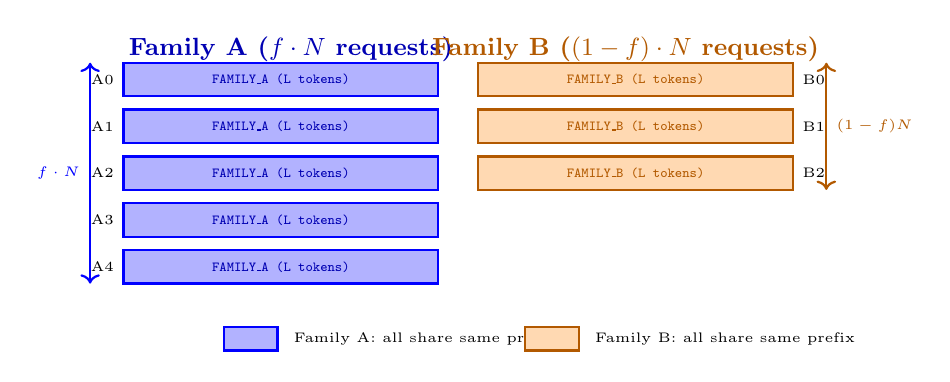
\begin{tikzpicture}[
    scale=0.85,
    every node/.style={font=\footnotesize}
]
% Parameters
\def\totalwidth{10}
\def\fraction{0.6}  % f = 0.6 (60% family A)
\pgfmathsetmacro{\halfwidth}{\totalwidth/2}
\pgfmathsetmacro{\leftwidth}{\halfwidth - 0.3}
\pgfmathsetmacro{\rightstart}{\halfwidth + 0.3}
\pgfmathsetmacro{\rightwidth}{\halfwidth - 0.3}
\def\boxheight{0.5}
\def\spacing{0.2}

% Title annotations
\node[font=\small\bfseries, blue!70!black] at (2.5, 2.5) {Family A ($f \cdot N$ requests)};
\node[font=\small\bfseries, orange!70!black] at (7.5, 2.5) {Family B ($(1-f) \cdot N$ requests)};

% Draw Family A requests
\foreach \i in {0,1,2,3,4} {
    \pgfmathsetmacro{\ypos}{1.8 - \i*(\boxheight + \spacing)}
    
    % Family A - all identical
    \fill[blue!30] (0, \ypos) rectangle (\leftwidth, \ypos + \boxheight);
    \draw[thick, blue] (0, \ypos) rectangle (\leftwidth, \ypos + \boxheight);
    
    % Label
    \node[left, font=\tiny] at (0, \ypos + \boxheight/2) {A\i};
    
    % Text inside
    \pgfmathsetmacro{\centerA}{\leftwidth/2}
    \node[blue!70!black, font=\tiny] at (\centerA, \ypos + \boxheight/2) {\texttt{FAMILY\_A (L tokens)}};
}

% Draw Family B requests
\foreach \i in {0,1,2} {
    \pgfmathsetmacro{\ypos}{1.8 - \i*(\boxheight + \spacing)}
    
    % Family B - all identical (but different from A)
    \fill[orange!30] (\rightstart, \ypos) rectangle (\totalwidth, \ypos + \boxheight);
    \draw[thick, orange!70!black] (\rightstart, \ypos) rectangle (\totalwidth, \ypos + \boxheight);
    
    % Label
    \node[right, font=\tiny] at (\totalwidth, \ypos + \boxheight/2) {B\i};
    
    % Text inside
    \pgfmathsetmacro{\centerB}{\rightstart + \rightwidth/2}
    \node[orange!70!black, font=\tiny] at (\centerB, \ypos + \boxheight/2) {\texttt{FAMILY\_B (L tokens)}};
}

% Annotations for counts
\pgfmathsetmacro{\topA}{1.8 + \boxheight}
\pgfmathsetmacro{\bottomA}{1.8 - 4*(\boxheight + \spacing)}
\draw[<->, thick, blue] (-0.5, \topA) -- (-0.5, \bottomA) 
    node[midway, left, font=\tiny] {$f \cdot N$};

\pgfmathsetmacro{\bottomB}{1.8 - 2*(\boxheight + \spacing)}    
\draw[<->, thick, orange!70!black] (\totalwidth + 0.5, \topA) -- (\totalwidth + 0.5, \bottomB) 
    node[midway, right, font=\tiny] {$(1-f) N$};

\fill[blue!30] (1.5, -2) rectangle ++(0.8, 0.35);
\draw[thick, blue] (1.5, -2) rectangle ++(0.8, 0.35);
\node[right, font=\tiny] at (2.4, -1.825) {Family A: all share same prefix};

\fill[orange!30] (6, -2) rectangle ++(0.8, 0.35);
\draw[thick, orange!70!black] (6, -2) rectangle ++(0.8, 0.35);
\node[right, font=\tiny] at (6.9, -1.825) {Family B: all share same prefix};

\end{tikzpicture}
\begin{itemize}
  \item Two large prefixes
  \item A fraction $f$ of the requests in a batch belong to family A, and the remaining requests belong to family $B$
\end{itemize}
\end{frame}

\begin{frame}{Two Family Batch Mixture (L = 2000 tokens)}
    \begin{figure}
        \centering
    \includegraphics[width=0.8\textwidth]{\RESULTDIR/two_family_fraction_A_2000.png}
    \captionof{figure}{Results across fraction of requests from A}
\end{figure}
\begin{itemize}
  \item All the prefill has already been completed so far
  \item Both the families are 2000 tokens in size
  \item Stark difference in throughput numbers between homogeneous and even slightly heterogeneous batches
\end{itemize}
\end{frame}

\begin{frame}{Two Family Mixture (L = 2000 tokens) - Mean DRAM Activity}
    \begin{figure}
        \centering
    \includegraphics[width=0.7\textwidth]{\RESULTDIR/mean_dram_act_frac_a_2000.png}
    \captionof{figure}{Mean DRAM Activity across fraction of requests from A (L = 2000 tokens)}
\end{figure}

\begin{itemize}
  \item DRAM activity higher for homogeneous batches
  \item Sequential accesses $\rightarrow$ more spatial locality  $\rightarrow$ higher prefetcher confidence $\rightarrow$ more requests issued $\rightarrow$ higher DRAM utilization
\end{itemize}
\end{frame}

\begin{frame}{Two Family Mixture (L = 2000 tokens) - Total DRAM Accesses}
    \begin{figure}
        \centering
    \includegraphics[width=0.7\textwidth]{\RESULTDIR/total_dram_acccesses_frac_a_2000.png}
    \captionof{figure}{Total DRAM Accesses across fraction of requests from A (L = 2000 tokens)}
\end{figure}

\begin{itemize}
  \item Total number of DRAM accesses lower for homogeneous batches
  \item Requests running in parallel $\rightarrow$ higher number of requests sharing the same block $\rightarrow$ better temporal locality $\rightarrow$ larger cache hit rates $\rightarrow$ less DRAM accesses
\end{itemize}
\end{frame}


\begin{frame}{Varying the amount of sharing}
\centering
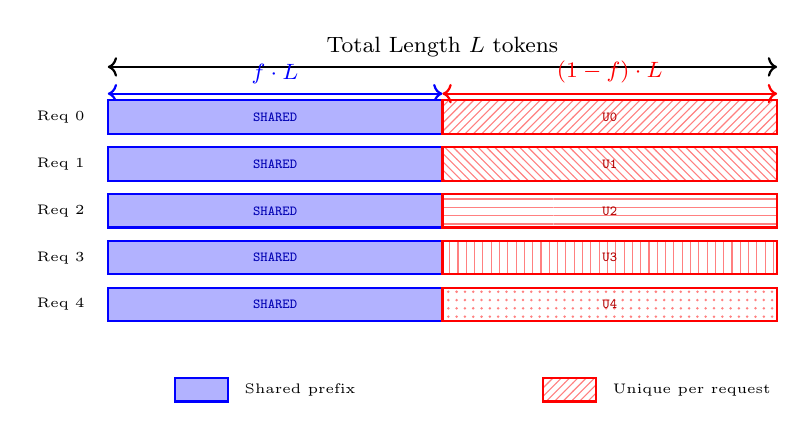
\begin{tikzpicture}[
    scale=0.85,
    every node/.style={font=\footnotesize}
]

\def\totalwidth{10}
\def\fraction{0.5} 
\pgfmathsetmacro{\sharedwidth}{\totalwidth * \fraction}
\pgfmathsetmacro{\uniquewidth}{\totalwidth * (1-\fraction)}
\def\boxheight{0.5}
\def\spacing{0.2}

\draw[<->, thick] (0, 2.2) -- (\totalwidth, 2.2) node[midway, above] {Total Length $L$ tokens};

\draw[<->, thick, blue] (0, 1.8) -- (\sharedwidth, 1.8) node[midway, above, blue] {$f \cdot L$};

\draw[<->, thick, red] (\sharedwidth, 1.8) -- (\totalwidth, 1.8) node[midway, above, red] {$(1-f) \cdot L$};

\foreach \i in {0,1,2,3,4} {
    \pgfmathsetmacro{\ypos}{1.2 - \i*(\boxheight + \spacing)}
    
    \fill[blue!30] (0, \ypos) rectangle (\sharedwidth, \ypos + \boxheight);
    \draw[thick, blue] (0, \ypos) rectangle (\sharedwidth, \ypos + \boxheight);
    
    \ifnum\i=0
        \fill[red!20, pattern=north east lines, pattern color=red!50] (\sharedwidth, \ypos) rectangle (\totalwidth, \ypos + \boxheight);
    \fi
    \ifnum\i=1
        \fill[red!20, pattern=north west lines, pattern color=red!50] (\sharedwidth, \ypos) rectangle (\totalwidth, \ypos + \boxheight);
    \fi
    \ifnum\i=2
        \fill[red!20, pattern=horizontal lines, pattern color=red!50] (\sharedwidth, \ypos) rectangle (\totalwidth, \ypos + \boxheight);
    \fi
    \ifnum\i=3
        \fill[red!20, pattern=vertical lines, pattern color=red!50] (\sharedwidth, \ypos) rectangle (\totalwidth, \ypos + \boxheight);
    \fi
    \ifnum\i=4
        \fill[red!20, pattern=dots, pattern color=red!50] (\sharedwidth, \ypos) rectangle (\totalwidth, \ypos + \boxheight);
    \fi
    \draw[thick, red] (\sharedwidth, \ypos) rectangle (\totalwidth, \ypos + \boxheight);
    
    \node[left, font=\tiny] at (-0.2, \ypos + \boxheight/2) {Req \i};
    
    \node[blue!70!black, font=\tiny] at (\sharedwidth/2, \ypos + \boxheight/2) {\texttt{SHARED}};
    \node[red!70!black, font=\tiny] at (\sharedwidth + \uniquewidth/2, \ypos + \boxheight/2) {\texttt{U\i}};
}


\fill[blue!30] (1, -2.8) rectangle ++(0.8, 0.35);
\draw[thick, blue] (1, -2.8) rectangle ++(0.8, 0.35);
\node[right, font=\tiny] at (1.9, -2.625) {Shared prefix};

\fill[red!20, pattern=north east lines, pattern color=red!50] (6.5, -2.8) rectangle ++(0.8, 0.35);
\draw[thick, red] (6.5, -2.8) rectangle ++(0.8, 0.35);
\node[right, font=\tiny] at (7.4, -2.625) {Unique per request};

\end{tikzpicture}

\vspace{0.3cm}
\end{frame}

\begin{frame}{Varying the amount of sharing (L = 500 tokens)}
    \begin{figure}
        \centering
    \includegraphics[width=0.7\textwidth]{\RESULTDIR/throughput_vs_amount_of_sharing_500_more_points.png}
    \captionof{figure}{Results across varying L}
\end{figure}

\begin{itemize}
  \item Initial throughput numbers quite low, because of lack of space in HBM
  \item $f$ increases $\rightarrow$ throughput increases
  \item A larger chunk shared $\rightarrow$ a larger duration of spatial and temporal locality
\end{itemize}
\end{frame}

\section{Key Idea}
\begin{frame}{Key Conclusions from the initial experiments}
  \begin{itemize}
    \item Memory requests from different requests are roughly simultaneous
    \item Sequential accesses are quite helpful to utilize DRAM bandwidth fully
    \item Enough requests should access nearby blocks to ensure high cache hit rates
    \item Batches should be completely homogeneous to utilize these benefits fully
    \item Merging requests from the same prefix together can also help in efficient KV cache eviction from the HBM $\rightarrow$ avoiding recomputation
  \end{itemize}
\end{frame}

\begin{frame}{Key Ideas and Metric Proposed}
  \textbf{Metric:} 
  \begin{itemize}
    \item (Number of requests running) $\times$ (Number of prefix chunks shared by \textbf{all} of them)
    \item Higher number of requests $\rightarrow$ efficient GPU utilization
    \item More number of prefix chunks shared $\rightarrow$ larger duration of spatial and temporal locality
    \item All requests $\rightarrow$ heterogeneous batches do not help
  \end{itemize}

  \textbf{Key Ideas:} 
  \begin{itemize}
    \item Efficiently compute shared chunks $\rightarrow$ \textbf{Chunked Hash Tree}
    \item Decision on when to stop the batch creation process $\rightarrow$ \textbf{RL}
  \end{itemize}
\end{frame}

\section{Chunked Hash Tree}
\begin{frame}{Chunked Hash Tree}
  \begin{itemize}
    \item Radix-tree selection is slow for large, online, long-context workloads
    \item Requests are represented using \textbf{hashed cumulative prefixes}
    \item Tokens are divided into fixed-size chunks
    \item Each level corresponds to \texttt{hash(tokens[0:k])}
    \item No explicit tree structure or node splitting
    \item Much faster than radix trees for large workloads
    \item Working set = set of active \textbf{(level, hash)} pairs
    \item Scheduling prefers requests with minimal missing chunks
  \end{itemize}
\end{frame}
\begin{frame}{Chunked Hash Tree - Insertion}
\centering
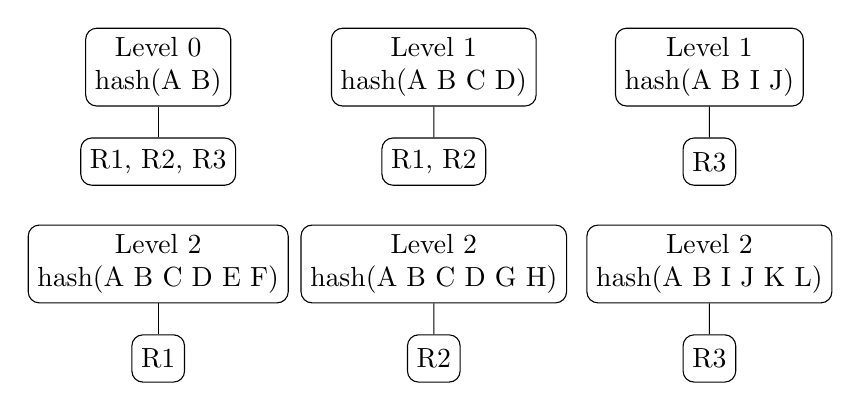
\begin{tikzpicture}[
    every node/.style={draw, rectangle, rounded corners, minimum height=6mm, align=center},
    level distance=12mm,
    sibling distance=32mm
]
\node (level0) at (0,0) {Level 0\\hash(A B)}
    child { node {R1, R2, R3} };
\node (level1) at (3.5,0) {Level 1\\hash(A B C D)}
    child { node {R1, R2} };
\node (level1) at (7,0) {Level 1\\hash(A B I J)}
    child { node {R3} };
\node at (0,-2.5) {Level 2\\hash(A B C D E F)}
    child { node {R1} };
\node at (3.5,-2.5) {Level 2\\hash(A B C D G H)}
    child { node {R2} };
\node at (7,-2.5) {Level 2\\hash(A B I J K L)}
    child { node {R3} };
\end{tikzpicture}
\vspace{0.5em}
\small
Each level stores hashes of cumulative token prefixes.
\end{frame}

\begin{frame}{Chunked Hash Tree - Working Set}
\centering
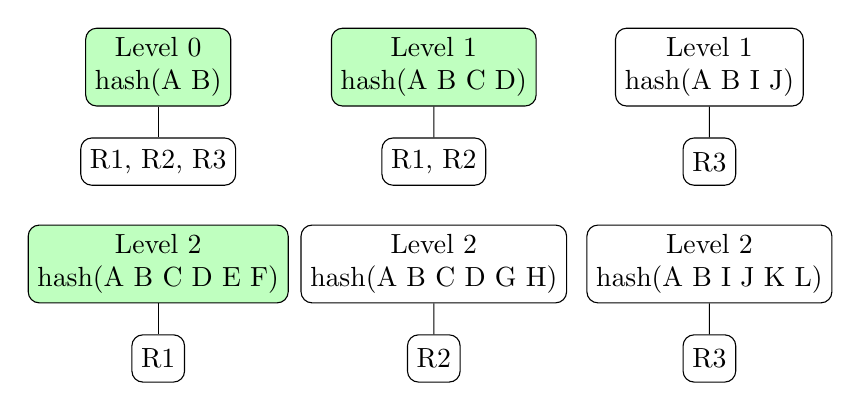
\begin{tikzpicture}[
    every node/.style={draw, rectangle, rounded corners, minimum height=6mm, align=center},
    ws/.style={fill=green!25},
    level distance=12mm,
    sibling distance=32mm
]
\node[ws] (level0) at (0,0) {Level 0\\hash(A B)}
    child { node {R1, R2, R3} };
\node[ws] (level1) at (3.5,0) {Level 1\\hash(A B C D)}
    child { node {R1, R2} };
\node (level1) at (7,0) {Level 1\\hash(A B I J)}
    child { node {R3} };
\node[ws] at (0,-2.5) {Level 2\\hash(A B C D E F)}
    child { node {R1} };
\node at (3.5,-2.5) {Level 2\\hash(A B C D G H)}
    child { node {R2} };
\node at (7,-2.5) {Level 2\\hash(A B I J K L)}
    child { node {R3} };
\end{tikzpicture}
\vspace{0.5em}
\small
Green boxes indicate prefix hashes in the working set.
\end{frame}

\begin{frame}{Chunked Hash Tree - Best Request Selection}
\centering
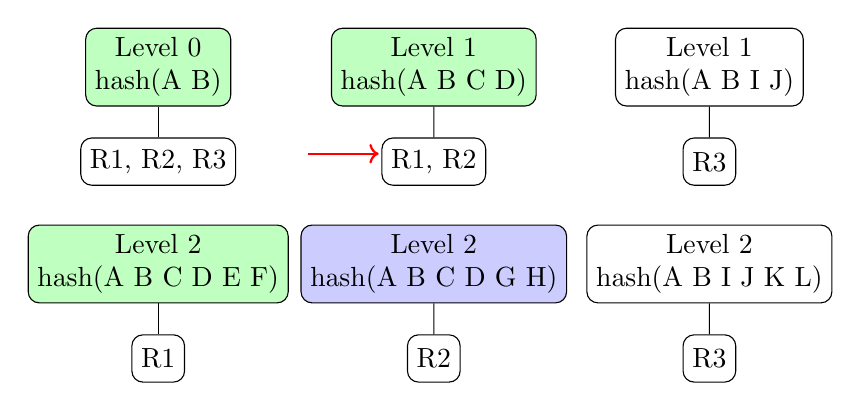
\begin{tikzpicture}[
    every node/.style={draw, rectangle, rounded corners, minimum height=6mm, align=center},
    ws/.style={fill=green!25},
    candidate/.style={fill=blue!20},
    level distance=12mm,
    sibling distance=32mm
]
\node[ws] (level0) at (0,0) {Level 0\\hash(A B)}
    child { node {R1, R2, R3} };
\node[ws] (level1) at (3.5,0) {Level 1\\hash(A B C D)}
    child { node {R1, R2} };
\node (level1) at (7,0) {Level 1\\hash(A B I J)}
    child { node {R3} };
\node[ws] at (0,-2.5) {Level 2\\hash(A B C D E F)}
    child { node {R1} };
\node[candidate] at (3.5,-2.5) {Level 2\\hash(A B C D G H)}
    child { node {R2} };
\node at (7,-2.5) {Level 2\\hash(A B I J K L)}
    child { node {R3} };
\draw[->, thick, red] (1.9,-1.1) -- (2.8,-1.1);
\end{tikzpicture}
\vspace{0.5em}
\small
Green boxes indicate prefix hashes in the working set. 

R2 is selected since it has maximum prefix overlap with the working set.
\end{frame}

\section{RL Decision Maker}
\begin{frame}{Formulation}
  \textbf{State:}
  \begin{itemize}
        \item \textbf{B:} current batch size
        \item $\mathbf{C_B:}$ number of chunks shared before adding a new request
        \item $\mathbf{C_A:}$ number of chunks which will remain shared after adding the new (best) request
        \item $\mathbf{R_W:}$ number of requests waiting at the end of $C_A$
    \end{itemize}

  \textbf{Action:}
  \begin{itemize}
        \item \textbf{ADD:} pop and activate the best request from the chunked hash tree
        \item \textbf{SKIP:} break the batch construction loop, dispatch the batch to GPU
    \end{itemize}

  \textbf{Reward:}
  \begin{itemize}
        \item Negative decode wall step time of the previous batch
        \item Delivered once per batch
    \end{itemize}
\end{frame}


\begin{frame}{Policies}
  \begin{itemize}
    \item \textbf{Q Learning:} The system tries actions (ADD or SKIP), observes rewards and gradually learns which action works best in each situation with respect to the long term outcome.
    \item \textbf{Contextual Bandit:} Which action works best right now (ignoring long-term future) in this situation?
    \item \textbf{Heuristics:} Based on current batch sizes and change in the number of chunks
  \end{itemize}
\end{frame}

\section{Results}
\begin{frame}{Throughput vs Req Rate (5 families) (Sequence Length: 3900 tokens)}
    \begin{figure}
        \centering
    \includegraphics[width=0.8\textwidth]{\RESULTDIR/throughput_across_req_rate_3.0.png}
    \captionof{figure}{Throughput vs Request Rate (5 families)}
\end{figure}
\end{frame}

\begin{frame}{Throughput vs Req Rate (5 families) (Sequence Length: 13000 tokens)}
    \begin{figure}
        \centering
    \includegraphics[width=0.8\textwidth]{\RESULTDIR/throughput_across_req_rate_10.0.png}
    \captionof{figure}{Throughput vs Request Rate (5 families)}
\end{figure}
\end{frame}

\section{}
\begin{frame}
    \Huge{\centerline{\bf Thank You}}
\end{frame}

\end{document}